\documentclass[Main]{subfiles}

\begin{document}


\section{Designprocess}

\subsection{Modtager}

Projektet skulle indeholde en sender som kunne sende kommandoer til dronen.

\begin{figure}[H]
\centering
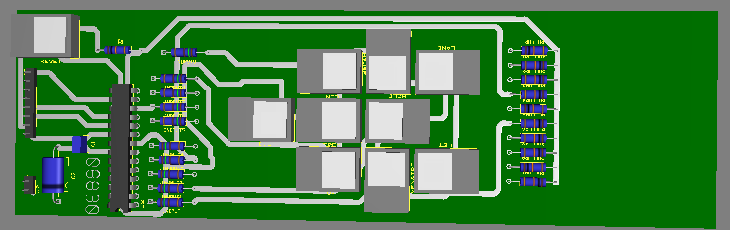
\includegraphics[width = 1 \textwidth]{3dUdenTal}
\caption{3D Figur af sender}
\label{Fig:3dUdenTal}
\end{figure}


Senderen er bygget op i form som en fjernbetjening, for at det er muligt at betjene den med en hånd.

Knapperne der er midt på printet er her brugeren giver sit input, som sendes videre.












\end{document}